%%%%%%%%%%%%%%%%%%%%%%%%%%%%%%%%%%%%%%%%%%%%%%%%%%%%%%%%%%%%%%%%%%%%%%%%%%%%%%%%
\section{SCENARIO 2: Both Hosts on Wi-Fi}
\label{sec:wifi}
\begin{figure}[h]
    \centering
    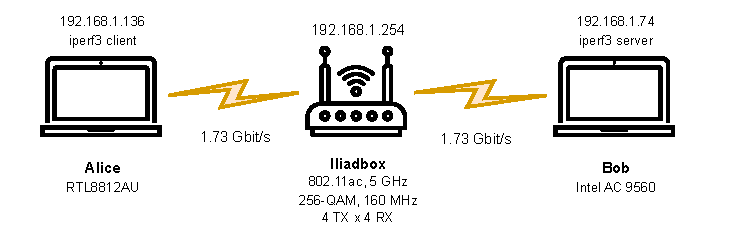
\includegraphics[width=0.95\linewidth]{images/wifi.drawio-3.pdf}
    \caption{Wi-Fi scenario}
    \label{fig:enter-label}
\end{figure}
\subsection{Scenario description}
For our second test, we benchmarked our LAN in the scenario of two hosts connected via Wi-Fi to the AP, far more common in the daily use of our home networks.

Using the same laptops as in the Ethernet test, now with Wi-Fi adapters, we configured the AP (same router as before) to enforce 802.11ac via the admin panel, from which we also confirmed it operated with 160 MHz channel bandwidth (eight 20 MHz channels combined) \cite{wikipedia_channelbonding} and 256-QAM modulation (combining amplitude and phase shifts to encode 8 bits in a symbol) \cite{wikipedia_qam}.

In this scenario, we had: Alice (\texttt{iperf3} client), IP: 192.168.1.136; Bob (\texttt{iperf3} server) with IP: 192.168.1.74.

\subsection{Computing the TMG}
Based on our information and on the router specifications (in particular, the number of antennas, which is 4 TX x 4 RX for the 5 GHz band), it has been easy to know about the capacity $C$ of the physical link in such a configuration \cite{wikipedia_80211ac}.
We have in fact a nominal capacity $C=1.73$ Gbit/s for both physical links, since both the clients are equipped with 2 TX x 2 RX antennas and support MU-MIMO. 

These numbers are to some degree confirmed by the statistics computed by the OS of our devices.
The TMG for the communication has been estimated using the equation:
\begin{align*}
    \text{TMG}&=\eta_{\text{TCPoHD}}\cdot\eta_{\text{802.11}}\cdot (0.5\cdot C)\\&=0.89\cdot 0.80\cdot (0.5\cdot1.73\text{ GBit/s)}=616\text{ Mbit/s}
\end{align*}
which takes into account the fact that every frame has to be transmitted twice (hence the factor 0.5), once from the sender to the AP and then from the AP to the recipient.
From the equations, TMG is 616 Mbit/s. We expect this to be valid for both directions ($A\to B$ and $B\to A$).

\subsection{Test results evaluation}
\begin{table}[htbp]
    \centering
    \caption{TCP Goodput from \texttt{iperf3} test (Mbps)}
    \label{tab:TCPoHD-throughput}
    \begin{tabular}{lrrrrc}
        \hline
        \textbf{Reverse flag} & \textbf{Avg} & \textbf{Median} & \textbf{Min} & \textbf{Max} & \textbf{Std Dev} \\
        \hline
        False & 192.0 & 193.5 & 177.0 & 197.0 & 5.42 \\
        True & 147.3 & 147.0 & 143.0 & 150.0 & 2.00 \\
        \hline
    \end{tabular}
\end{table}

The test results clash with our expectations; in fact, we have a third of the \text{TMG} in the direction $A\to B$ and even a lower goodput for the direction $B\to A$. 
We dived deeper in the specifications of all the devices, discovering that the RTL8812AU chipset is only capable of exploiting channel bandwidths up to 80 MHz. Our estimation needs now to take into account the disparity in the speeds of the two links, with the ${A\leftrightarrow AP}$ link being the bottleneck. In particular, the overall capacity is not anymore $0.5\cdot C$, since the two channels have different transmission speeds:
\begin{itemize}
    \item $C_{A\leftrightarrow AP}= C/2 = 867$ Mbit/s
    \item $C_{B\leftrightarrow AP}= C = 1.73$ Gbit/s
\end{itemize}
% \begin{equation}
% \begin{cases}
%     T_{\text{data, C1}}&=\frac{\sub{MSS}{TCPoHD}}{\sub{TMG}{802.11, C1}}=\frac{1460\ \text{B}}{867\ \text{Mbit/s}}=13.5\ \si{\micro\second}\\
%     T_{\text{overhead, C1}}&=\frac{\sub{Header}{TCPoHD}+\sub{Header}{IP}+\sub{Overhead}{Eth}}{\sub{TMG}{802.11, C1}}\\&=\frac{20+20+38\ \text{B}}{867\ \text{Mbit/s}}=0.72\ \si{\micro\second}\\
%     T_{\text{data, C2}}&=\frac{\sub{MSS}{TCPoHD}}{\sub{TMG}{802.11, C2}}=\frac{1460\ \text{B}}{1.73\ \text{Gbit/s}}=6.75\ \si{\micro\second}\\
%     T_{\text{overhead, C2}}&=\frac{\sub{Header}{TCPoHD}+\sub{Header}{IP}+\sub{Overhead}{Eth}}{\sub{TMG}{802.11, C1}}\\&=\frac{20+20+38\ \text{B}}{1.73\ \text{Gbit/s}}=0.36\ \si{\micro\second}\\
%     \eta_\text{links}&=\frac{T_{\text{data, C2}}}{T_{\text{data, C1}} + T_{\text{data, C2}} + T_{\text{overhead, C1}} + T_{\text{overhead, C2}}}=32\%\\
%     G&= \eta_\text{links}
% \cdot\eta_{\text{TCPoHD}}\cdot\eta_{\text{802.11}}\cdotC_{\text{802.11},\ A\leftrightarrow AP}}
% \end{cases}
% \end{equation}
Let $C'$ be the new overall capacity. Then:
\begin{equation*}
\begin{cases}
    C'&=\frac{\text{Data}}{\text{TX Time}}=\frac{\text{Data}}{\text{TX Time }(A\leftrightarrow AP)\ +\ \text{TX Time }(AP\leftrightarrow B)}
    \\&=\frac{\text{Data}}{\frac{\text{Data}}{C_{A\leftrightarrow AP}}+\frac{\text{Data}}{C_{B\leftrightarrow AP}}}
    \\&=\frac{1}{1/C_{A\leftrightarrow AP}\ +\ 1/C_{B\leftrightarrow AP}}=\frac{1}{3}\cdot C=578\text{ Mbit/s}\\
    \text{TMG}&= \eta_{\text{TCPoHD}}\cdot\eta_{\text{802.11}}\cdot C'\\&=0.89\cdot0.80\cdot578\text{ Mbit/s}=411\text{ Mbit/s}
\end{cases}
\end{equation*}
The new equations estimate a TMG of 411 Mbit/s, but discrepancies from the results persist, likely due to signal attenuation, interference from neighbour networks, and unknown device limitations. 

Similar to Ethernet, we also have to tackle the loss of goodput (-23\%) when communicating in the $B\to A$ direction with respect to the $A\to B$ direction. We are unsure on what caused the discrepancy, which is nonetheless consistent across several tests. While the reciprocity principle \cite{balanis2005antenna} suggests symmetrical TX/RX performance, real antennas include additional components that may introduce asymmetries.
We hypothesize that 802.11ac optimizes the downlink, as switching to 802.11n @ 2.4 GHz reversed the effect. No other configuration adjustments (client-server swap, device variation, UDP use) made the trend change.

As seen in the Ethernet scenario, we now examine the sequence number and goodput graphs for this case as well. In this PCAP instance, we observe that no retransmissions occurred. 
\begin{figure}[H]
    \centering
    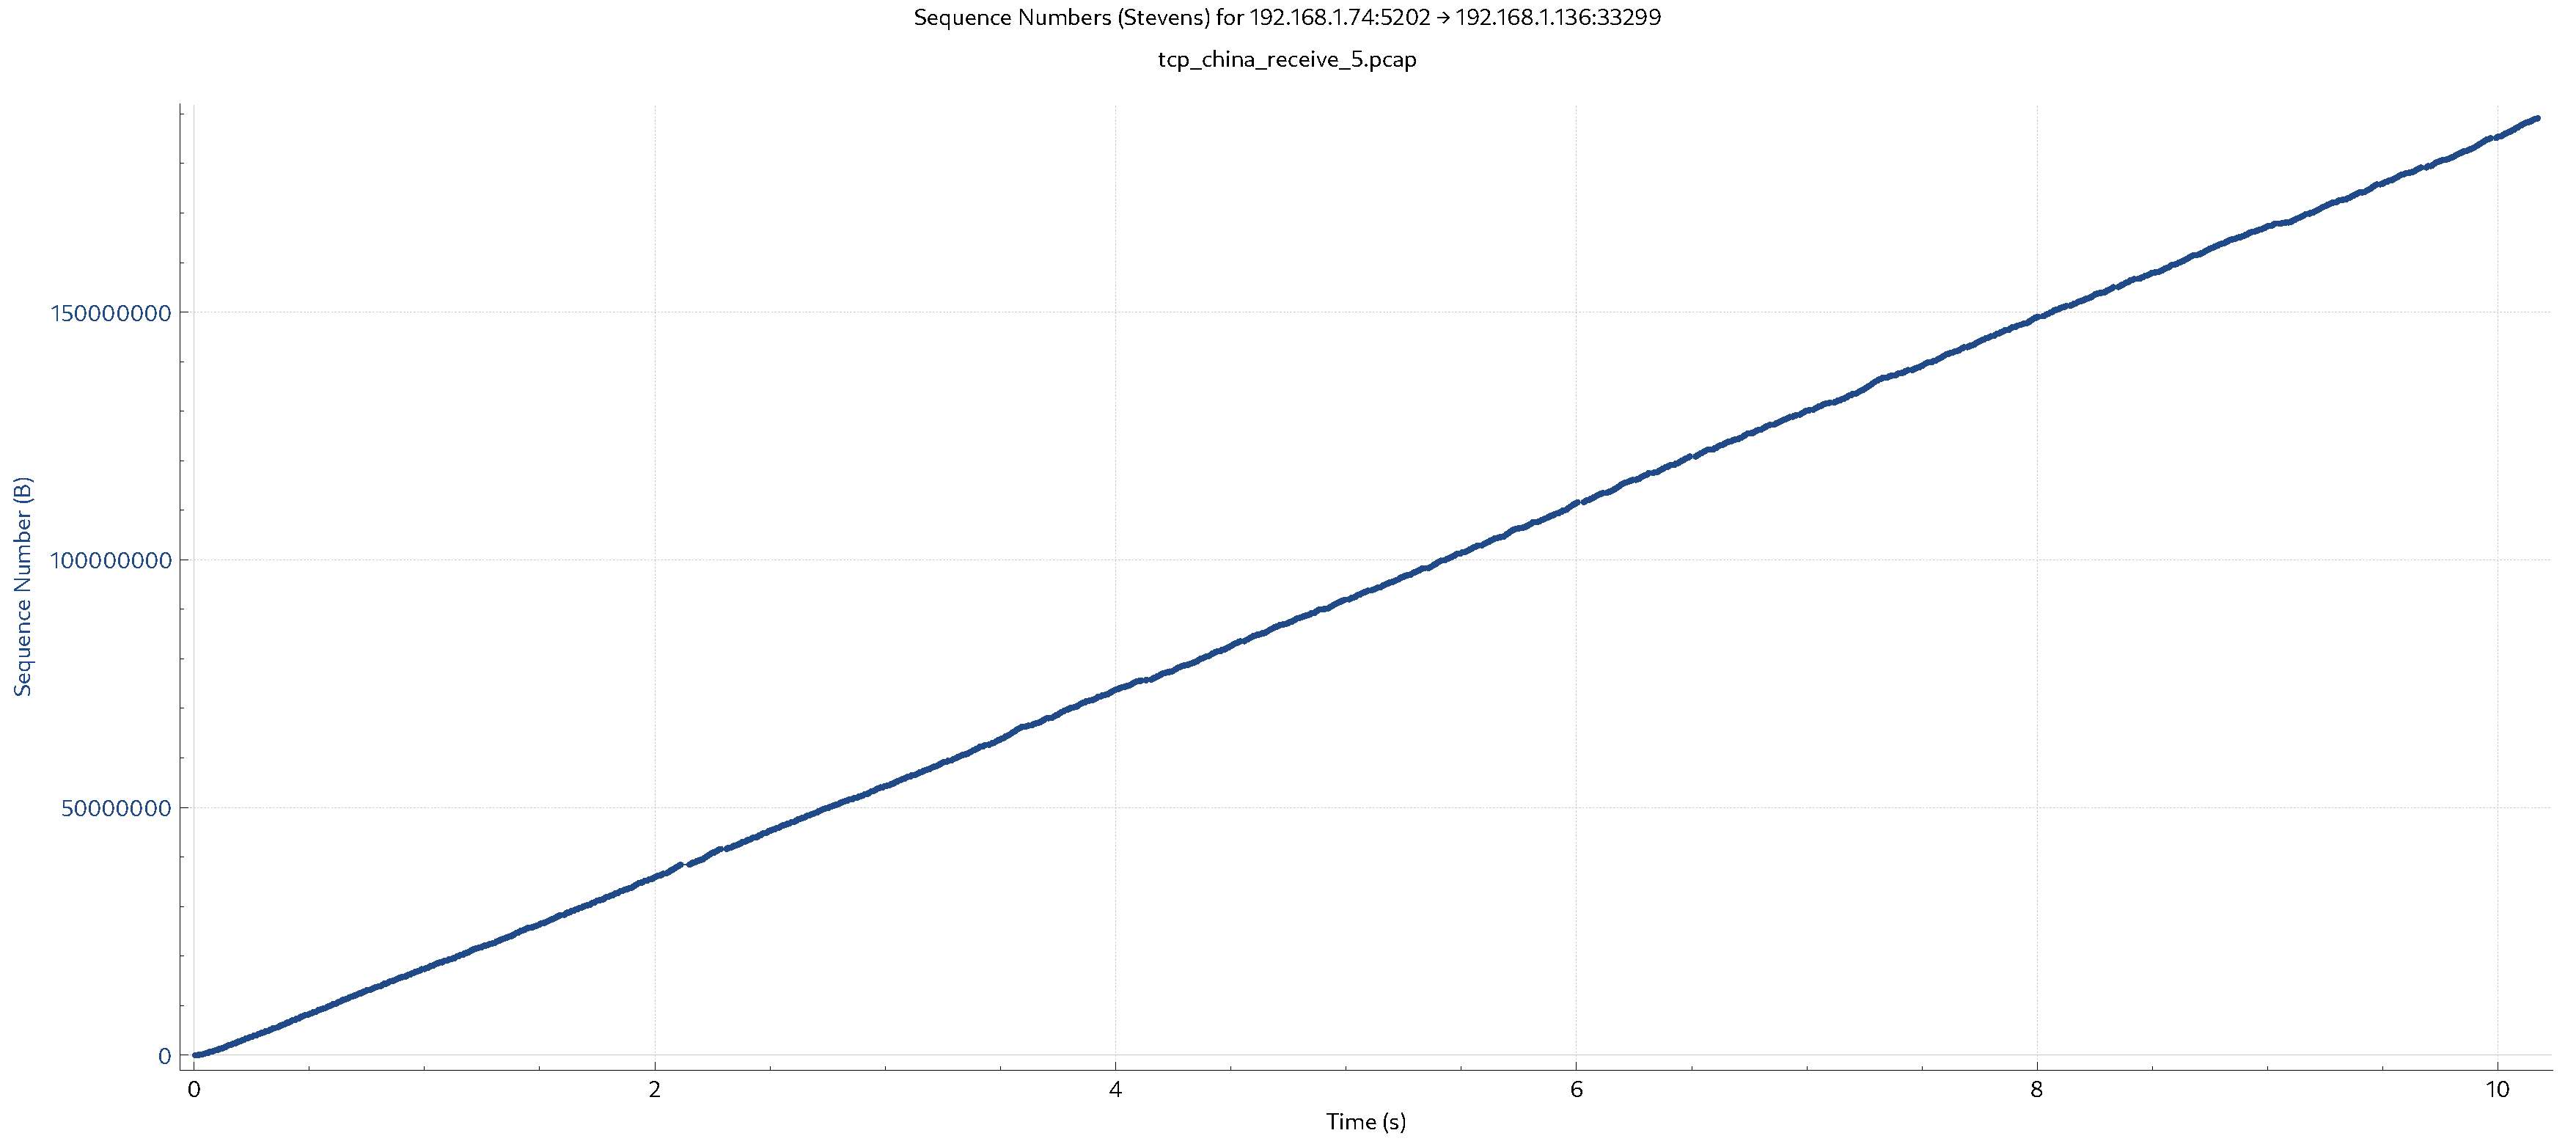
\includegraphics[width=0.75\linewidth]{images/SeqNumberChina.pdf}
    \caption{Sequence Numbers (Stevens), reverse flag set to True}
    \label{fig:enter-label}
\end{figure}

However, unlike the Ethernet scenario, the goodput shows more fluctuation over time (it is no longer a flat, horizontal line but displays small oscillations), indicating the presence of a less stable wireless channel. 

\begin{figure}[H]
    \centering
    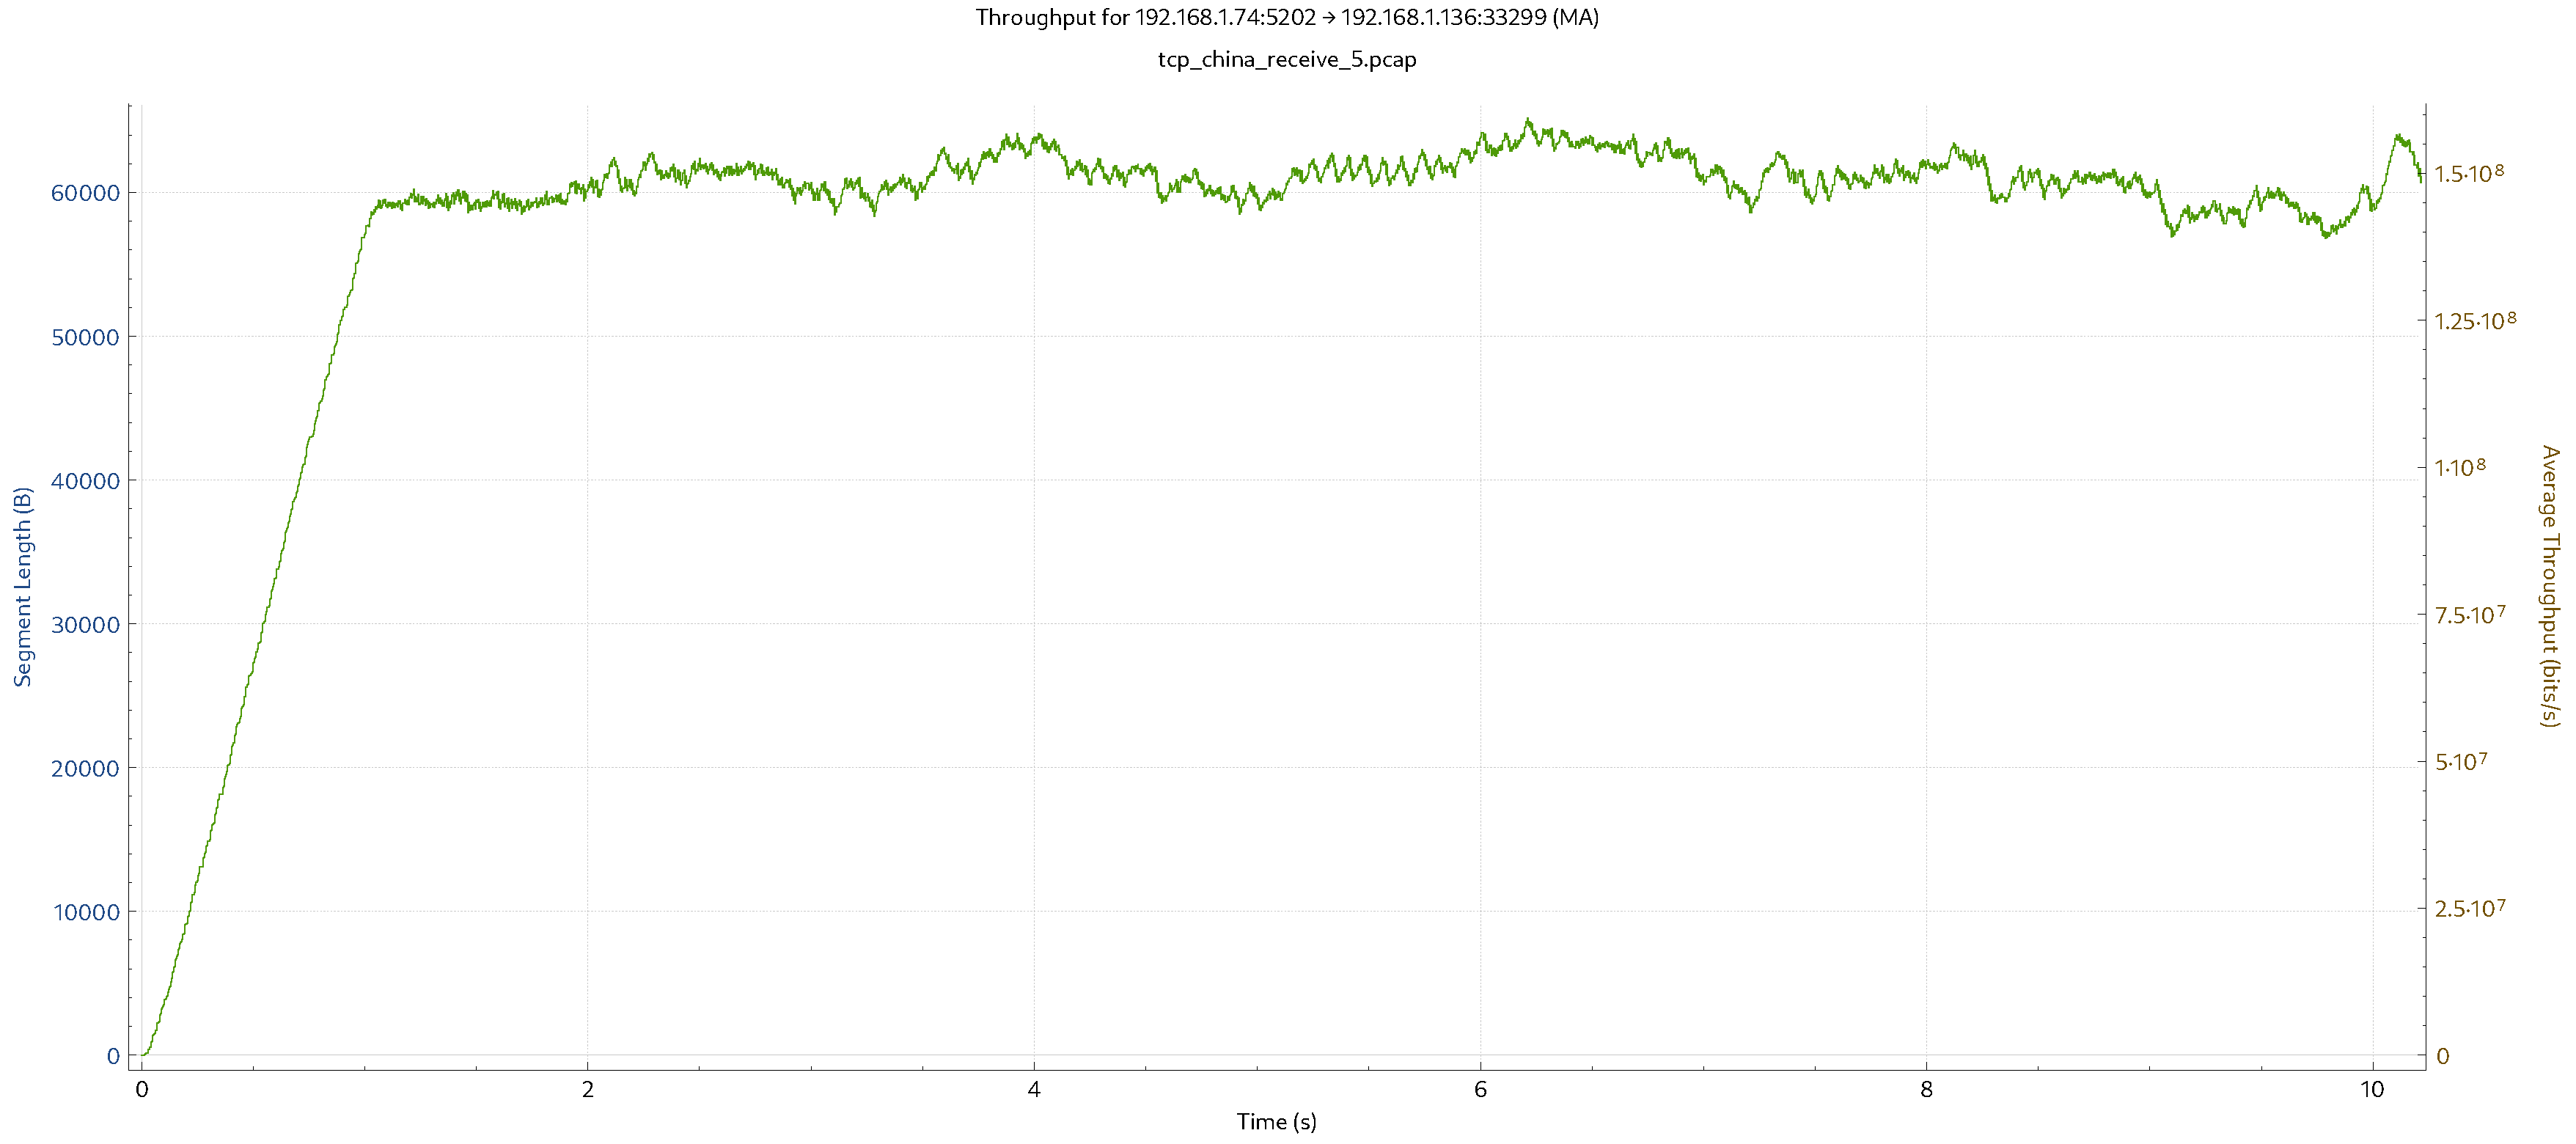
\includegraphics[width=0.75\linewidth]{images/GoodputChina.pdf}
    \caption{Goodput (MA) on the receiver side, reverse flag set to True}
    \label{fig:enter-label}
\end{figure}

The goodput is also significantly lower than in the Ethernet case.
The average goodput calculated from the different \texttt{iperf3} tests is 147.3 Mb/s, which closely matches the value observed on Wireshark (above 150 Mb/s, as shown in the graph). The slight discrepancy can be attributed to the seventh test, which performed worse than the others (with retransmissions observed), causing a drop in the overall average goodput.